\subsection*{Proposed architecture}
Similar to time-domain direct-form IIR filter design, which relies on feeding back the filter's recursive part with a combination of delayed instances of its output (see Figure \ref{fig:IIR_feedbachArch}), our approach relies on spatial feedback of received array signals back to the transmitter.
\begin{figure}[!h]
\begin{center}
\includegraphics[width=0.5\linewidth]{./Media/BASIC_IIR_FILTER_ARCH.png}
\caption{Direct form IIR architecture. This architecture is based on feeding the input to the recursive part with delayed and weighted instances of its output.}
\label{fig:IIR_feedbachArch}
\end{center}
\end{figure}
In order to do so, we propose a dual beam-former architecture (see Figure \ref{fig:Proposed_spatialIIR_ARCH}), defined by two sets of spatial weights $\vecnot{\alpha},\vecnot{\beta}$, generating two independently spatially filtered signals $\vecnot{\alpha}^{T}\Steer{\theta_{g}},\vecnot{\beta}^{T}\Steer{\theta_{g}}$. One is the system's output and the other is fed back to the medium using a transmitting antenna.
\begin{figure}[!h]
\begin{center}
\includegraphics[width=0.75\linewidth]{./Media/SpatialIIR-diagram/SpatialIIR_VER5.pdf}
\caption{The proposed ``dual beam-former`` architecture. One beam-former, $\vecnot{\alpha}$, is generates the output signal. The other $\vecnot{\beta}$ synthesize the feedback transmission.}
\label{fig:Proposed_spatialIIR_ARCH}
\end{center}
\end{figure}
\subsection*{The proposed system's spatial response}
Time domain analysis of the proposed feedback based architecture, considering both propagation delay and attenuation, gives rise to
\begin{equation}
    \label{eqn:SingleSensorTemporalEquality}
    % \resizebox{.91\linewidth}{!}{
        \begin{split}
            x_{n}(t) = g\rBrace{s\rBrace{t-\tau_{pd}-\tau_{n}}
            +\sum_{m=0}^{N-1}{\alpha_{m}x_{m}\rBrace{t-\tau_{pd}-\tau_{n}}}},
        \end{split}
    % }
\end{equation}
where the first term of the right-hand side represents the contribution of the transmitted waveform $s(t)$ to the $n$'th array element and the second term represents the feedback contribution of the re-transmitted array signal to this same element.
Expressing \eqref{eqn:SingleSensorTemporalEquality}'s Fourier transform,
\begin{equation}
    \label{eqn_singleSensorFourier}
    % \resizebox{.91\linewidth}{!}{
        \begin{split}
            \F{x}_{n}\rBrace{\omega} =
            g\Bigg( & \F{s}\rBrace{\omega}
            \exp\rBrace{-j\omega\rBrace{\tau_{pd}+\tau_{n}}}
            \\&+\sum_{m=0}^{N-1}
            {
            \alpha_{m}\omegaB\F{x}_{m}\rBrace{\omega}
            \exp\rBrace{-j\omega\rBrace{\tau_{pd}+\tau_{n}}}
            }\Bigg),
        \end{split}
    % }
\end{equation}
and its vector from,
$$
\F{\vx}\rBrace{\omega} = ge^{-j\omega\tau_{pd}} \rBrace{\F{s}\rBrace{\omega}+\vAlphaT \F{\vx}\rBrace{\omega}}\vd,
$$
we find that it can be simplified to
$$
\F{\vx}\rBrace{\omega} =\rBrace{I-g\vd\vAlphaT{}e^{-j\omega\tau_{pd}}}^{-1}g\vd\exp{\rBrace{-j\omega\tau_{pd}}}\F{s}\rBrace{\omega}.
$$
Then, denoting
\[
\phi\triangleq\omega\tau_{pd}
\]
as the round-trip signal propagation related electrical phase and using the Woodbury matrix identity \cite{woodbury1950inverting}, we find that
$$
\F{\vx}\rBrace{\omega}
=
\frac{    
g\vd\exp{\rBrace{-j\phi}}
}{
1 - g\aTd{}\exp{\rBrace{-j\phi}}
}\F{s}\rBrace{\omega}.
$$
Considering the noiseless case $\rBrace{\text{i.e. n}\rBrace{t}=0}$,
we express the general spatial response of FB as 
\begin{equation}
\label{eqn:GeneralFeedbackTransferFunction}
\Hba
\triangleq
\frac{\F{z}\rBrace{\omega}}{\F{s}\rBrace{\omega}} 
=
\frac{    
g\bTd{}\exp\rBrace{-j\phi}
}{
1 - g\aTd{}\exp\rBrace{-j\phi}
}.
\end{equation}
\par Note that this result confirms that the suggested architecture achieves a controllable (via setting of $\vBeta$ and $\vAlpha$) and recursive (non-trivial denominator) spatial response.
As will be shown, high directivity and narrow beam-width are obtainable by proper selection of the weights. Comparing to traditional beamformers (i.e. with no feedback), the performance improvement will be expressed in terms of aperture increase, computing the traditional beamformer aperture which achieves the same performance.
One may observe that opposed to traditional beamformers, the beampattern, $\Hba,$ is not only influenced by the impinging signal DOA, for it is also range selective due to its $\phi$ dependency.
As exemplified in Fig.~\ref{fig_rangeAzimuthSelectivity}, the combination of both angular and range selectivity enables the designer to enhance signals arriving from specific locations rather than only specific directions.
\begin{figure}[t!]
    \begin{center}
        \begin{overpic}[width=0.65\linewidth, 
        % grid, 
        tics=10,trim=0 0 0 0]{./Media/azimuthRangSelectivity.png}
            \put (20, 23){\rotatebox{0}{\footnotesize{Angular response}}}
            \put (30.5, 47){\rotatebox{0}{\footnotesize{Enhanced radial slice}}}
        \end{overpic}
    \end{center}
     \caption{A visualization of the spatial area selectivity concept. Combining both radial selectivity (i.e. enhancing signals from a specific distance) and DOA-based selectivity, allows the enhancement of signals arriving from specific areas (grey filled), while signals originated in other areas (even from the same DOA) are suppressed.}
    \label{fig_rangeAzimuthSelectivity}
\end{figure}
\section{Fisher information matrix}
A possible evaluation for the contribution of the presented feedback mechanism is to measure the additional information in the system.
To this end, the FIM, denoted by $J$, will now be calculated with respect to the DOA parameter $\thetaD$ and the range related parameter $\phi$. 
As the feedback-based transfer function (\ref{eqn:GeneralFeedbackTransferFunction}) is expressed in frequency domain, we rely on \cite{zeira1990frequency} to express the frequency domain FIM as well. 
\par A single FIM element, may be expressed as
\begin{equation}\label{eq_FIM_kl_full}
    \resizebox{.9\linewidth}{!}{
        \begin{split}
            J_{\vBrace{k,l}}\rBrace{\vEta} 
            =&
            \Re\cBrace{
            \frac{1}{2\pi}
            \int_{-\omega_{s}/2}^{\omega_{s}/2}
            {
            \frac{1}{\Phi\rBrace{\omega}}
            \mathfrak{F}^{*}\left\{
            \frac{\partial z(t)}{\partial\eta_{k}}
            \right\}
            \mathfrak{F}\left\{
            \frac{\partial z(t)}{\partial\eta_{l}}
            \right\}
            d\omega
            }}
            \\ &+
            \frac{T}{4\pi}
            \int_{-\omega_{s}/2}^{\omega_{s}/2}
            \frac{1}{\Phi^{2}\rBrace{\omega}}
            \frac{\partial\Phi\rBrace{\omega}}{\partial\eta_{k}}
            \frac{\partial\Phi\rBrace{\omega}}{\partial\eta_{l}}
            d\omega
        \end{split}
    }
\end{equation}
where $ \vEta = [\thetaD,\phi]^{T} $ is the parameters vector, $\Re$ stands for the real-part extraction operator, $k,l \in\cBrace{1,2}$, $\Phi\rBrace{\omega}$ is the noise spectrum, $\mathfrak{F}$ is the Fourier transform operator, $T$ is the measurement observation interval and $\omega_{s}$ is the signal bandwidth. 
For simplicity, $\text{n}\rBrace{t}$ is assumed to be a white Gaussian with some constant power spectral density $\Phi(\omega)=\sigma^2$ and independent of the estimated parameters $\eta$, hence the second term vanishes. 
Assuming continuously differentiable functions, where order alteration of the Fourier transform and the differentiation operations is allowed, \eqref{eq_FIM_kl_full} simplifies to
\begin{equation}
    \label{eq_beamPatternFreqDomain_FIM}
    % \resizebox{1\linewidth}{!}{
        \begin{split}
            J_{\vBrace{k,l}}\rBrace{\vEta} = 
            \Re\cBrace{
            \frac{1}{2\pi\sigma^2}
            \int_{-\omega_{s}/2}^{\omega_{s}/2}
            {
            \rBrace{\frac{\partial{}\F{z}\rBrace{\omega}}{\partial\eta_{k}}}^{\ast}
            \frac{\partial{}\F{z}\rBrace{\omega}}{\partial\eta_{l}}
            d\omega
            }}
        \end{split}.
    % }
\end{equation}
As mentioned before, $g$ is independent of the estimated parameters, therefore
\begin{equation}\label{eq_vdDiff}
\frac{\partial\vd}{\partial\thetaD}=A\omegaB\vd
\end{equation}
where $A\omegaB$ is an $N\times{}N$ diagonal matrix and each of its diagonal elements may expressed as 
\[
A_{\vBrace{i,i}}\omegaB=-j\omega\frac{\partial \tau_{i}}{\partial{\thetaD}}\ \  \forall{i\in\cBrace{0\hdots{}N-1}}.
\]
To further simplify the analysis, without loss of generality, we use (in this section only) $g=1$.
In App.~\ref{apdx_clacFim} we compute the FIM terms, concluding that
\begin{equation}
    \label{eqn_FIMelements}
    \resizebox{.91\linewidth}{!}{
        \begin{split}
            &J_{\theta\theta}
            =
            \frac{1}{2\pi\sigma^{2}}\int_{-\omega_{s}/2}^{\omega_{s}/2}{\frac{
            \lBrace{\vBetaT{}A\omegaB\vd-\vBetaT{}B\omegaB\vAlpha\ePhi{-}}^{2}
            }{
            \lBrace{\rBrace{1-\aTd\ePhi{-}}^{2}}^{2}
            }\lBrace{\F{s}\rBrace{\omega}}^{2}d\omega}
            \\
            &J_{\phi\phi}
            =
            \frac{1}{2\pi\sigma^{2}}\int_{-\omega_{s}/2}^{\omega_{s}/2}{\frac{
            \lBrace{\bTd}^{2}
            }{
            \lBrace{\rBrace{1-\aTd\ePhi{-}}^{2}}^{2}
            }\lBrace{\F{s}\rBrace{\omega}}^{2}d\omega}
        \end{split}
    }
\end{equation}
where $B\omegaB\triangleq\vd\vdT{}A\omegaB-A\omegaB\vd\vdT$.
Moreover, using some mild assumptions and setting
\begin{equation}\label{eq_alphaBetaPropSteer}
    \vAlpha,\vBeta\propto\vd^{\ast},
\end{equation}
we show that the cross terms of the FIM are nullified, i.e. $J_{\theta\phi} = J_{\phi\theta}^{*}=0$.
\par 
Choosing the weights as in \eqref{eq_alphaBetaPropSteer} may be interpreted as a generalization of the DS beamformer, formerly referenced as the conventional beamformer (CB) \cite{van2004optimum}, which coherently integrate the impinging signal along the array elements.
The same choice of weights also minimizes the $\lBrace{1-\aTd\ePhi{-}}$ term, significantly increasing the available information, as predicted by the FIM.
It is worth mentioning that \eqref{eq_vdDiff} is relevant even for arbitrary (non-omni-directional) sensors when smooth and slowly changing radiation patterns are assumed.
In practice, though, there will be unavoidable errors, and perfect knowledge of the steering vector $\vd$ is not always available.
In Sec.~\ref{sec_Performance}, we quantify the effect of such estimation errors and discuss its influence on the array performance. 
\section{Performance of array processing with feedback}
In this section we analkyze some of the frundamental properties of an array; it's beamwidth and it's peak to a sidelobe level. As we show, by integrating the feedback, we can obtain performance much better than the classic  beamforming. We analyze the performance for general manifold, and then show the obtained results for a ULA. 
\subsection{Array beamwidth}
Many approaches may be considered while setting $\vecnot{\alpha},\vecnot{\beta}$ in order to achieve optimal utilization of the spatial IIR structure in (\ref{eqn:GeneralFeedbackTransferFunction}), all sharing the same purpose of minimizing the IIR component (i.e. the denominator) for specific spatially selected signals.
One naturally considered approach is the \textbf{dual-conventional-beamformer} (DCBF). In this approach, to achieve minimization of the IIR component,$ \vecnot{\beta}^{T}\vecnot{d}_{\theta_{s}}e^{-j\omega\tau_{s}} = 1 $ (where $\tau_{s}$ is determined by the target's location), in order to achieve the desired high spatial selectivity. Considering the array phase and gain mismatch, we present $\rho = re^{\Phi}$, which will function as the \textbf{array-mismatch-factor}. Combined with the \textbf{conventional beamformer} (\cite{VanTrees2002DetectionIV}) we set $ \vecnot{\alpha} = \vecnot{\beta} = \frac{\rho}{N}\vecnot{d^{*}_{s}e^{-j\tau_{s}}} $). Comparing the perfectly-aligned scenario $\left(\theta = \theta_{s}, \tau = \tau_{s}\right)$ with the general scenario, enables calculation of the half-power-beamwidth (\textbf{HPBW}) by setting $\left|\frac{H_{\theta_{s}\tau_{s}}\left(\omega{}\right)}{H_{\theta,\tau}\left(\omega{}\right)}\right|^{2} = 2$, which translates to 
\begin{align}
\label{eqn_arrPerformance_beamwidth_3dB}
\Hr{\theta}{\tau}{}
\triangleq
\fbBpRatio
=
2\ .
\end{align}
Defining $\D{N}{x} = \frac{\sin{Nx}}{\sin{x}}$ , and performing some algebraic simplification, one gets
\ifdefined\showDev
    \\
    \fbox{
    \begin{minipage}{.95\linewidth}
    \textbf{development specifics}
    $$
    \Hr{\theta}{\tau}{}
    =
    \left|
    \frac{
    \vecnot{\alpha}^{T}\vecnot{d}_{\theta_{s}}
    }{
    \vecnot{\alpha}^{T}\vecnot{d}_{\theta}
    }
    \frac{
    1-\vecnot{\beta}^{T}\vecnot{d}_{\theta}e^{-j\tau}
    }{
    1-\vecnot{\beta}^{T}\vecnot{d}_{\theta_{s}}e^{-j\tau_{s}}
    }
    \right|
    =
    \left|
    \frac{
    1
    }{
    \frac{1}{N}\vecnot{d}^{H}_{\theta_{s}}\vecnot{d}_{\theta}
    }
    \frac{
    1-\frac{\rho}{N}\vecnot{d}^{H}_{\theta_{s}}\vecnot{d}_{\theta}e^{j\Delta_{\tau}}
    }{
    1-\rho
    }
    \right|
    $$
    .Using the geometric progression sum of the steering vectors product,
    $$
    \vecnot{d}^{H}_{\theta_{s}}\vecnot{d}_{\theta} = \Sigma_{n=0}^{N-1}e^{j\left(\theta-\theta_{s}\right)}
    $$
    and defining $\Delta_{\theta} \triangleq \theta-\theta_{s}$ one gets
    $$
    \vecnot{d}^{H}_{\theta_{s}}\vecnot{d}_{\theta} = e^{j\frac{N-1}{2}\Delta_{\theta}}\D{N}{\dTheta}
    $$.
    Integrated into the last expression, it yields\\
    \resizebox{.95\linewidth}{!}{
    \begin{minipage}{\linewidth}
    \begin{align*}
    \left|
    \frac{
    1
    }{
    1-\rho
    }
    \frac{
    N-\rho\vecnot{d}^{H}_{\theta_{s}}\vecnot{d}_{\theta}e^{j\Delta_{\tau}}
    }{
    \vecnot{d}^{H}_{\theta_{s}}\vecnot{d}_{\theta}
    }
    \right|^{2}
    &=
    \left|
    \frac{
    1
    }{
    1-\rho
    }
    \left(
    N\Dp{N}{\dTheta/2}{-1}
    e^{-j\frac{N-1}{2}\Delta_{\theta}}
    - 
    \rho{}e^{j\Delta_{\tau}}
    \right)
    \right|^{2}
    \\&=
    \left|
    \frac{
    1
    }{
    1-\rho
    }
    \left(
    N\Dp{N}{\dTheta/2}{-1}
    - 
    \rho{}e^{j\left(\Delta_{\tau}+\frac{N-1}{2}\Delta_{\theta}\right)}
    \right)
    \right|^{2}
    \\
    &=
    \frac{1}{\left|1-\rho\right|^{2}}
    \left(
    N^{2}\Dp{N}{\dTheta/2}{-2}
    -2rN\Dp{N}{\dTheta/2}{-1}\cos{\left(\Phi+\Delta_{\tau}+\frac{N-1}{2}\Delta_{\theta}\right)}
    +r^{2}
    \right)
    \end{align*}
    \end{minipage}}
    \\
    where $ \Delta_{\tau} \triangleq \tau-\tau_{s}$
    \end{minipage}
    }
\else
\fi
\resizebox{.97\linewidth}{!}{
  \begin{minipage}{\linewidth}
      \begin{align}
        \nonumber
        \label{eqn_arrayPerformance_beamwidth_fullEpxr}
        \Hr{\theta}{\tau}{2}
        =
        \frac{1}{\left|1-\rho\right|^{2}}
        \Bigg(
        & 
        N^{2}\Dp{N}{\dTheta/2}{-2} 
        \\ \nonumber &
        - 2rN\Dp{N}{\dTheta/2}{-1}\cos{\left(\Phi+\Delta_{\tau} + \frac{N-1}{2}\Delta_{\theta}\right)}
        \\ & 
        + r^{2}\Bigg),
    \end{align}
  \end{minipage}
}
where $ \Delta_{\tau} \triangleq \tau-\tau_{s} $ and $ \Delta_{\theta} \triangleq \theta-\theta_{s}$.
which can be easily verified to tend to $ 1 $ when $ \Delta_{\tau},\Delta_{\theta} \rightarrow 0$. 
Following \cite{VanTrees2002DetectionIV}'s steps (discussed in section \ref{section_arrayPerformance_classicULA}), we start by investigating the first order taylor expansion,$$ \evalat{f\left(x,y\right)}{x\to{}a,y\to{}b} \approx f(a,b) + \evalat{\frac{\partial{f}}{\partial{x}}}{\left(x=a,x=b\right)}\left(x-a\right) + \frac{\partial{f}}{\partial{x}}\left(a,b\right) $$,of the expression.
Using L'Hôpital's rule to evaluate the derivatives, results in 
\resizebox{.97\linewidth}{!}{
  \begin{minipage}{\linewidth}
    \begin{align*}
        \Hr{\theta}{\tau}{2}
        \propto &
        1 
        \\ &
        - \left(r\left(N-1\right)\sin{\Delta_{\tau}}\right)\Delta_{\theta}
        \\ &
        -\left(2Nr\mathcal{D}^{-1}\left(N,\sfrac{\Delta}{2}\right)\sin{\left(\frac{N-1}{2}\frac{\Delta_{\theta}}{2}\right)}\right)\Delta_{\tau}.
    \end{align*}
  \end{minipage}
}
Observing that setting $\Delta{\tau},\Delta{\theta} = 0$ zeros the first order coefficients, leads us to express the second order terms, resulting in 
\resizebox{.97\linewidth}{!}{
  \begin{minipage}{\linewidth}
    \begin{align}
        \label{eqn_arrayPerformance_beamwidth_approx}
        \nonumber
        \Hr{\theta}{\tau}{2} 
        \approx 
        1
        +
        \frac{1}{\left|1-\rho\right|^{2}}
        \Bigg(&
        \frac{1}{12}\left(N-1\right)\left(\left(1+2r\right)N-4r+1\right)\Delta^{2}_{\theta}
        \\& \nonumber
        + r\Delta^{2}_{\tau}
        \\&
        + r\left(N-1\right)\Delta_{\theta}\Delta_{\tau}
        \Bigg).
    \end{align}
  \end{minipage}
}
\begin{figure}
    \todo{Refine graph (units , labels, title)}
    \label{fig_singleFreqFeedback_2ndTaylorNumericalValidation}
    \centering
    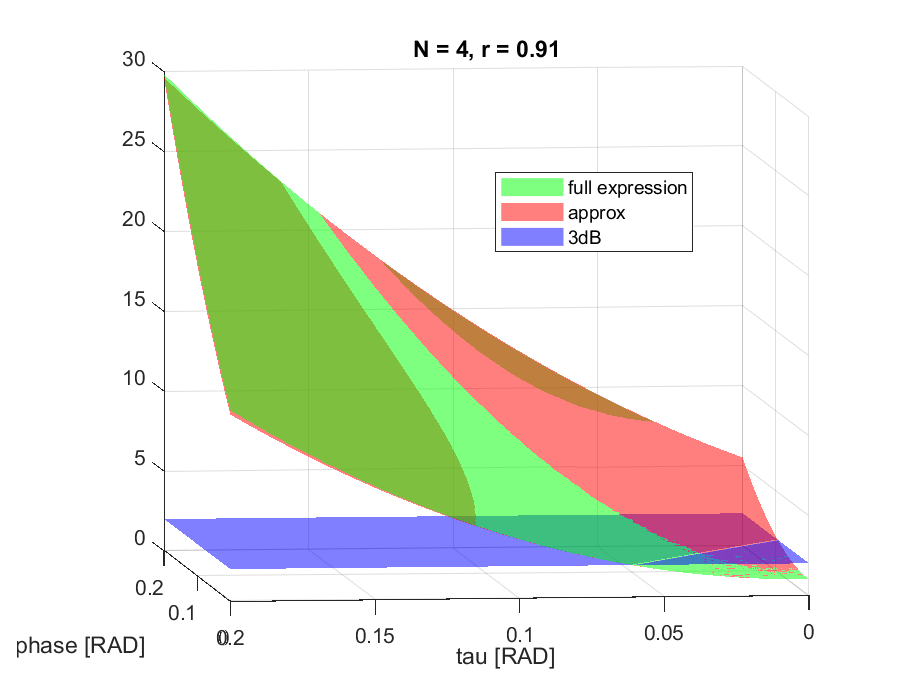
\includegraphics[width=0.9\linewidth]{./Media/spatial_IIR_MATLAB/beamwidth/BW_approx_validation.eps}
    \caption{Graphically comparing (\ref{eqn_arrayPerformance_beamwidth_fullEpxr}) and (\ref{eqn_arrayPerformance_beamwidth_approx}) for $N=4$ and $\rho=0.91$. The approximation seems to closely match the original expression.}
\end{figure}
Unlike the passive ULA case, it is evident from figure (\ref{fig_singleFreqFeedback_2ndTaylorNumericalValidation}) that the $4^{th}$ order terms are not needed for the evaluation of $\theta_{HPBW}$. In perfect phase alignment (i.e. $\Delta_{\tau}=0$), the u-space expression for the HPBW is $$u_{HPBW} =
\frac{
\left|1-\rho\right|
}{
\pi{d}
}
\lambda
\sqrt{\frac{
12
}{
\left(N-1\right)\left(\left(1+2r\right)N-4r+1\right)
}}.
$$
Comparing to the classic ULA beamwidth \cite{VanTrees2002DetectionIV}, thoroughly discussed in appendix \ref{appendix_theULABeamwidth}, we can express the improvement factor as
$$
\frac{
0.89\frac{\lambda}{ND}
}{
\theta_{HPBW,IIR}
}
=
\frac{0.89}{\left|1-\rho\right|}\sqrt{\frac{1+2r}{12}}
$$
\todo{TODO}
\textbf{Add graph of the improvement factor}
% \subsection{The pole-based design approach}
% In this approach, we look for setting the response "poles" which minimize the denominator, thus maximizing the overall response magnitude. To evaluate the beamwidth, we chose to allocate all of the system's poles in a single position such that 
% $
% 1-\vecnot{\beta}^{T}\vecnot{d}_{\theta}e^{-j\tau}
% =
% \left(e^{j\theta}-re^{j\theta_{s}}\right)^{N}
% $
% where $N$ is the number of array sensors and $r \in \left[0,1\right)$ enables us to avoid treatment of $\infty$-valued expressions. Next, we look for $\theta$ such that
% $
% \left|\frac{
% \frac
% {
% \vecnot{\alpha}^{T}\vecnot{d}_{\theta_{s}}
% }{
% \vecnot{\beta}^{T}\vecnot{d}_{\theta_{s}}
% }
% }{
% \frac
% {
% \vecnot{\alpha}^{T}\vecnot{d}_{\theta}
% }{
% \vecnot{\beta}^{T}\vecnot{d}_{\theta}
% }
% }\right|
% = \frac{1}{\sqrt{2}}
% $. Assuming that, like in classical IIR filter design theory, the numerator behaviour is significantly "slower" than the denominator's which results in $\vecnot{\alpha}^{T}\vecnot{d}_{\theta} 
% \approx
% \vecnot{\alpha}^{T}\vecnot{d}_{\theta_{s}}$ reults in
% \begin{align*}
%     \left|\frac{
%     \vecnot{\beta}^{T}\vecnot{d}_{\theta}
%     }{
%     \vecnot{\beta}^{T}\vecnot{d}_{\theta_{s}}
%     }\right|
%     &= \frac{1}{\sqrt{2}}
%     \\
%     \left|
%     \frac{
%     \left(e^{j\theta}-re^{j\theta}\right)^{N}
%     }{
%     \left(e^{j\theta}-re^{j\theta_{s}}\right)^{N}
%     }
%     \right|
%     &=
%     \left|
%     \frac{
%     \left(1-re^{j\left(\theta_{s}-\theta\right)}\right)
%     }{
%     \left(1-r\right)
%     }
%     \right|^{N}
%     \\
%     &=
%     \left|
%     \frac{
%     1+r^{2}-2r\cos{\left(\theta_{s}-\theta\right)}
%     }{
%     \left(1-r\right)^{2}
%     }
%     \right|^{\frac{N}{2}}
%     =
%     \left(\frac{1}{2}\right)^{\frac{1}{2}}
%     \\
%     \Rightarrow 
%     1+r^{2}-2r\cos{\left(\theta_{s}-\theta\right)}
%     &=
%     \left(1-r\right)^{2}2^{\frac{1}{N}}
%     \\
%     \cos{\left(\theta_{s}-\theta\right)}
%     &=
%     \frac{
%     1+r^{2}-\left(1-r\right)^{2}2^{\frac{1}{N}}
%     }{
%     2r
%     }
%     \\
%     \Rightarrow
%     \frac{\omega{D\left(cos(\theta_{g,s})-cos(\theta_{g,B})\right)}}{c}
%     &=
%     cos^{-1}
%     \left(
%     \frac{1+r^{2}-\left(1-r\right)^{2}2^{\frac{1}{N}}}{2r}
%     \right)
% \end{align*}.
% Therefore,
% \begin{equation}
%     \theta_{g,B} 
%     &= 
%     cos^{-1}
%     \left(
%     cos(\theta_{g,s})
%     -
%     \frac{c}{\omega{D}}
%     cos^{-1}
%     \left(
%     \frac{1+r^{2}-\left(1-r\right)^{2}2^{\frac{1}{N}}}{2r}
%     \right)
%     \right)
% \end{equation}
% Few observations can be derived from the $ \theta_{g,B} $:
% \begin{itemize}
%     \item $r\rightarrow{1}$ (i.e. setting the pole on the unit circle) causes $\theta_{g,B}\rightarrow\theta_{g,s}$ due to the $\infty$ valued response at $\theta_{g,s}$
%     \item The interval 
%     $
%     \left\{
%     \theta_{g,s}
%     \ \Bigg{|}\ 
%     cos(\theta_{g,s})
%     -
%     \frac{c}{\omega{D}}
%     cos^{-1}
%     \left(
%     \frac{1+r^{2}-\left(1-r\right)^{2}2^{\frac{1}{N}}}{2r}
%     \right)
%     <-1
%     \right\}
%     $, has no solution. In simulations, when evaluating such $\theta_{g,s}$ values, one can observe that the actual beampattern does not resemble the designed one due to the ULA geometric properties.
%     \item The number of sensors $N$ seems to have low impact on the beamwidth.
% \end{itemize}
\subsection*{Phase alignment sensitivity}
Although (\ref{eqn_arrayPerformance_beamwidth_fullEpxr})'s high sensitivity (see (\ref{eqn_arrayPerformance_beamwidth_approx})) to $\dTheta$ expresses the desirable ``sharp`` spatial IIR beampattern, it's high sensitivity to $\dTau$, as will be demonstrated, states that only target which reside in a very impractically specific range (i.e. $\tau$) will be enhanced. To evaluate the necessary accuracy, we compare $\Hr{\theta}{\tau}{2}$ to $2$, while setting $\dTheta=0$ (i.e. perfectly steered array). It follows that $$\frac{r}{\left|1-\rho\right|^{2}}\dTau^{2} = 1,$$ i.e. only a very small range interval $\Delta{R} \triangleq \frac{\dTau}{2\pi{}\lambda}$ is amplified. Setting typical physical parameters (both in RF or acoustic environments) result in $\Delta{R} \propto 10^{-4}_{\left[m\right]}$ which is obviously impractical, considering array ambiguity, signal modeling errors, range estimation errors etc.